\documentclass[a4paper]{article}
\usepackage[margin=2cm]{geometry}
\usepackage{graphicx}
\usepackage{wrapfig}
\usepackage{array}
\graphicspath{ {/} }
\author{Ayush Agarwal}
\begin{document}
\begin{center}
 \huge\textbf{Ayush Agarwal}\\
\end{center}
\hrule
\section*{}
\begin{wrapfigure}{r}{0.20\textwidth} 
    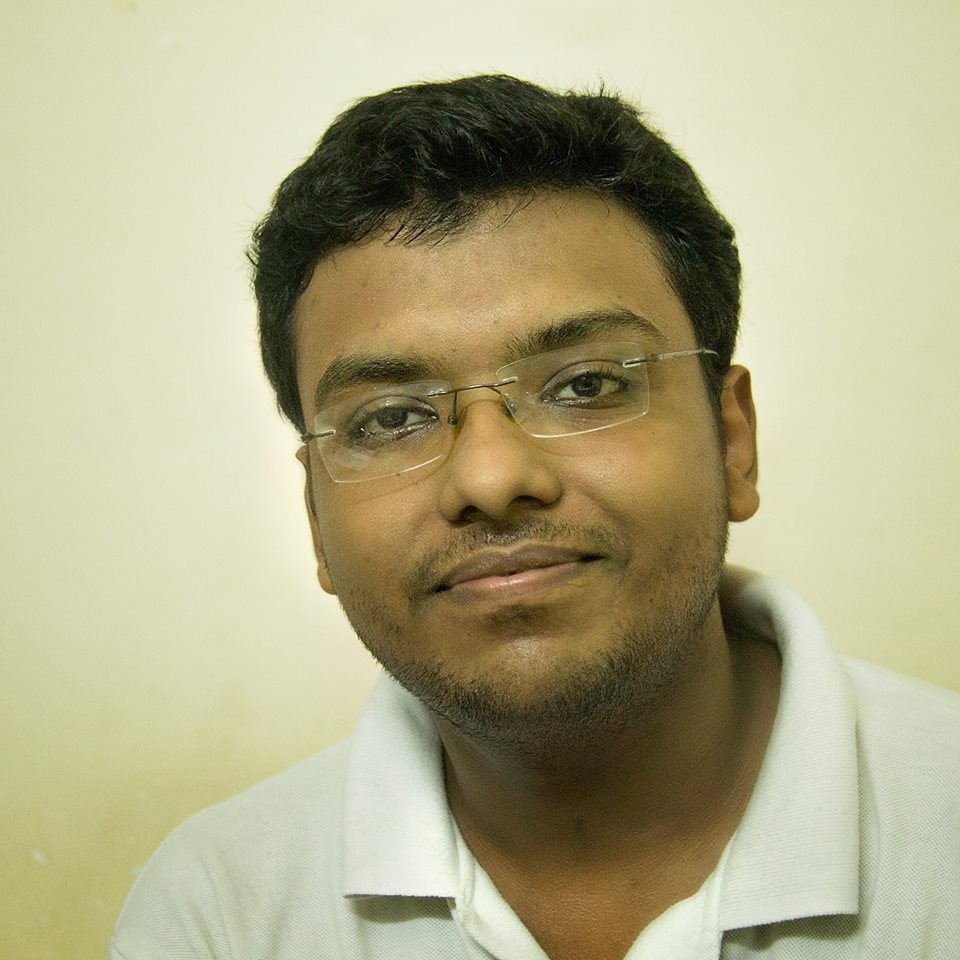
\includegraphics[width=0.20\textwidth]{photo}
\end{wrapfigure}
 Sophomore Undergraduate,\\
 Computer Science and Engineering,\\
 IIT Kanpur.\\
 \\
 $8090686935$\\
 $ayushaga@iitk.ac.in$\\
 \vspace{10mm}
 %%%%%%%%%%%%%%---Education---%%%%%%%%%%%%%%%%%%%%%%%%%%
 \section*{Education}
 \hrule
 \begin{center}
 \vspace{3mm}
  \begin{tabular}{|c|c|c|c|}
  \hline
  Year & Degree & Institute & CPI\\
  \hline
  2017(Expected)& B.Tech, Computer Sc.&IIT Kanpur&$8.7/10$\\
  \hline
  2013& HSCE&St.Anselm's Sr. Sec. School&89\% \\
  \hline
  2011& AISSE&St.Anselm's Sr. Sec. School&10/10 \\
  \hline
  \end{tabular}
 \end{center} 
  
%%%%%%%%%%%%%%%%%%--Achievements----%%%%%%%%%%%%%%%%%%%
 \section*{Achievements}
 \hrule
 \vspace{3mm}
  \begin{itemize}
   \item AIR-146 in JEE-Advance, 2013.	
   \item Scored 325/360 marks in JEE-Mains 2013.
   \item NTSE and KVPY Scholar 
   \item Rank-1 in International Mathematics Olympiad(IMO) by SOF.
   \item Among final 35 students selected for OCSC Camp for International Physics Olympiad(IPhO),2013 .
  \end{itemize}
 
 
%%%%%%%%%%%%%%%%----Projects---%%%%%%%%%%%%
\section*{Projects}
\hrule
\vspace{3mm}
  \begin{itemize}
   \item 
   \textbf{Portal for Academic Mentor System for Counselling Service,IITK}
	   \begin{itemize}
	    \item A portal using JS , php and mysql for a better interaction of core team, academic mentors and academically 
		  deficient students.Used codeignitor (a php framework) for MVC (Model View Controller system) 
		  and bootstrap for designing.
	   \end{itemize}
    \item
      \textbf{Application on Delaunay  Triangulation}
	\begin{itemize}
	 \item A python gui using Scipy,Tkinter,Numpy and Opengl. 
	      Given an image as an input it used to convert it into an image made from very small triangles.
	\end{itemize}
  \end{itemize}

  
 %%%%%%%%%%%%%%%%--------Technical Skills--------%%%%%%%%%%%%%
 \section*{Technical Skills}
 \hrule
 \vspace{3mm}
  \begin{tabular}{@{}m{4.0cm}m{13cm}@{}}
   \textbf{\textrm{Languages}} & 
C, C$++$, Python, Php, Dart\\
    
  \textbf{\textrm{Platforms}} &
  Linux, Windows\\
  
  \textbf{\textrm{Tools}} &
  HTML, CSS, SCSS, JavaScript, Git, Angular-Dart, Angular-JS\\
  \end{tabular}



\end{document}

